\chapter{\IfLanguageName{dutch}{Proof Of Concept}{Proof Of Concept}}%
\label{ch:proofofconcept}

In dit stukje gaat er stap per stap beschreven worden hoe de testapplicatie zal worden opgebouwd. Deze zal een handleiding bevatten om de applicatie ook zelf te kunnen ontwikkelen, en er is ook een link naar de GitHub-Repository \footnote{GitHub Repo: \url{https://github.com/EmilioTR/kalenderapplicatie}.} van de volledig afgewerkte applicatie beschikbaar.


\section{Voorbereiden}

Voor dat we beginnen met de applicatie te ontwikkelen is het eerst belangrijk om vast te leggen welke requirements erin gaan zitten en hoe de kalender er gaat uitzien qua lay-out. \newline

Met behulp van de lijst met eisen verkregen door de MoSCoW-methode, is het nu eenvoudig te bepalen welke onderdelen in de applicatie worden opgenomen. We zullen alle 'must-haves' en 'should-haves' integreren, met uitzondering van 'notificaties' en 'prioritering van taken'. Deze twee functies worden uitgesloten omdat een notificatiesysteem voor deze proof of concept niet noodzakelijk is, en omdat de implementatie van taakprioritering meer tijd in beslag zou nemen dan nodig is om een testbare applicatie te ontwikkelen. Het is een functie die later nog altijd kan worden toegevoegd.\newline

Nu we weten welke functies we willen implementeren, kunnen we beginnen met het ontwerpen van de lay-out van de applicatie. Het ontwerp moet eenvoudig, overzichtelijk en gebruiksvriendelijk zijn. Om dit te bereiken, zullen we een beperkt aantal grote en duidelijke knoppen gebruiken. De hele functionaliteit moet intuïtief zijn, zodat gebruikers er gemakkelijk mee overweg kunnen en hun doelen kunnen bereiken met een minimaal aantal klikken. Dit kan worden bereikt door de belangrijkste functies op één scherm te plaatsen, zonder het te druk te maken. \newline

Om dit te bereiken en het overzichtelijk te houden, kunnen we hulpmiddelen gebruiken zoals een dialoogvenster voor het beheren van evenementen en een zijmenu ("drawer") voor extra functies zoals een "Brain Dump".  \newline

Door het gebruik van sobere kleuren blijft de app rustig en aangenaam om naar te kijken. De categorie kleuren daarentegen mogen sterk van contrast zijn om zo een duidelijk verschil te geven tussen het soort evenementen, wat ook helpt bij het overzicht en de duidelijkheid van alles dat is ingepland. \newline

Voor een eerste visuele weergave van het ontwerp worden er mock-up’s gemaakt (zie Figuur 4.1 en 4.2). De verkozen themakleur is pastelviolet, deze is zeer neutraal en zorgt voor een rustige omgeving.

\begin{figure}[h]
    \centering
    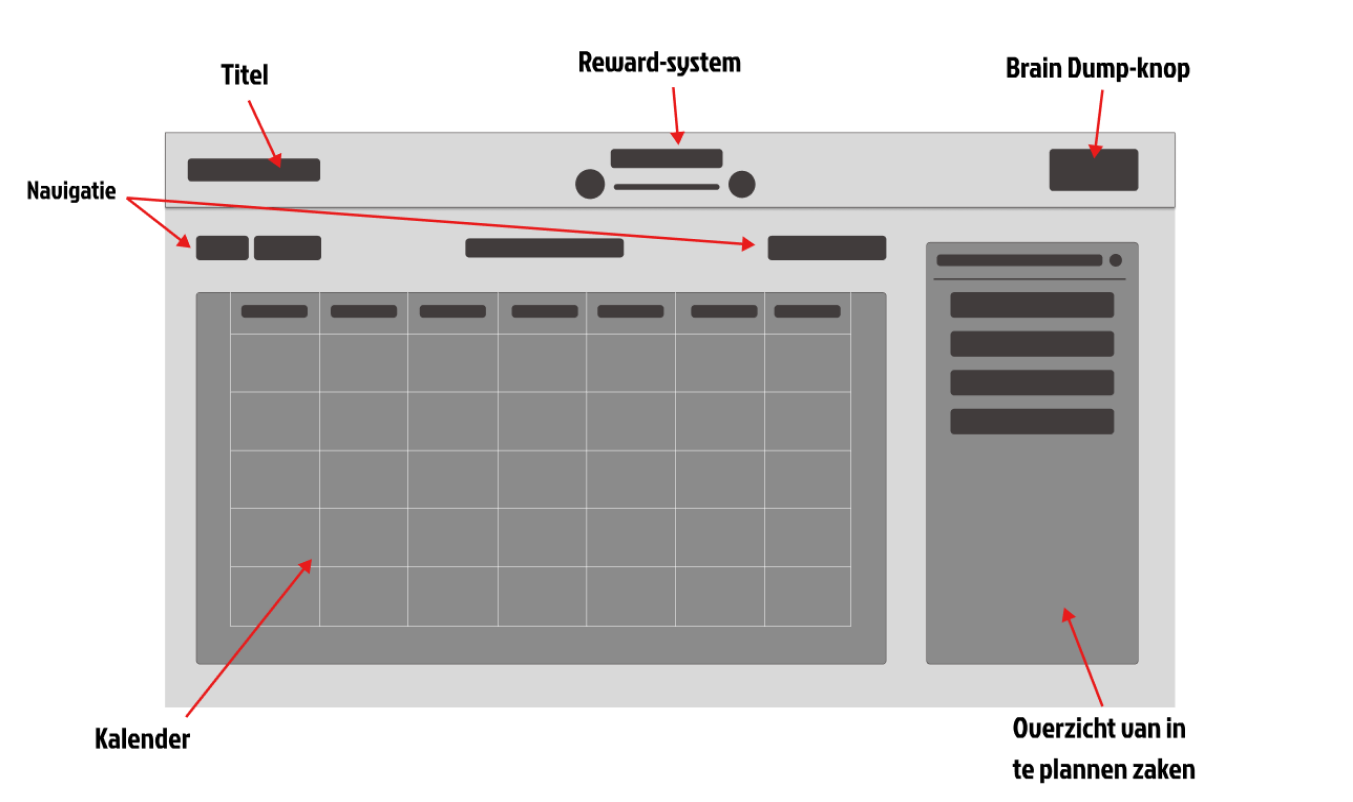
\includegraphics[width=\textwidth]{graphics/mockup_kalender.png}
    \caption{Mockup van de kalenderapplicatie.}
    \label{fig:mockup_app}
\end{figure}

\begin{figure}[h]
    \centering
    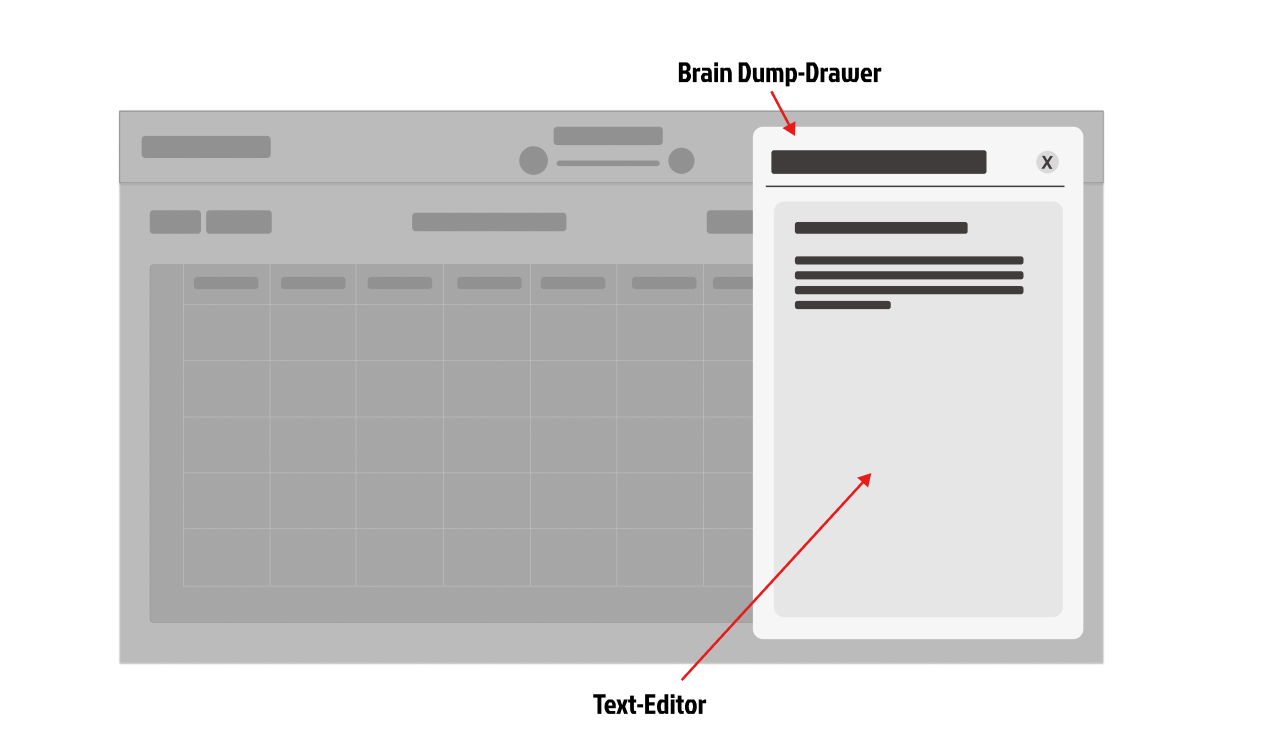
\includegraphics[width=\textwidth]{graphics/mockup_braindump.png} 
    \caption{Mockup van de Brain Dump functie.}
    \label{fig:mockup_braindump}
\end{figure}


\section{Opbouw van de applicatie}

De Proof of Concept zal worden ontwikkeld als een webapplicatie, wat de bruikbaarheid en implementatie ervan aanzienlijk vergemakkelijkt. De keuze voor het ontwikkelingsframework valt op 'Next.js', een veelgebruikt JavaScript-framework voor het bouwen van “single page applications”. En als IDE zal er gekozen worden voor Visual Studio Code. \newline

De beslissing om voor Next.js te kiezen komt voort uit verschillende overwegingen. Allereerst maakt Next.js het zeer eenvoudig om de applicatie online te hosten dankzij de ingebouwde server-side rendering. Bovendien vereenvoudigt het framework het beheer van de backend, wat van cruciaal belang kan zijn in latere ontwikkelingsfasen, vooral als er met een database moet worden geïntegreerd.  \newline

Hoewel deze proof of concept geen backend zal hebben en er geen permanente gegevensopslag naar een database zal plaatsvinden, zal alles operationeel zijn met testgegevens uit een JSON-bestand. Echter biedt het gebruik van Next.js de flexibiliteit om in de toekomst eenvoudig over te schakelen naar een meer geavanceerde backend-architectuur, mocht dat nodig zijn.

\subsection{Vereisten voor de ontwikkeling}

Om een applicatie te kunnen maken in Next.js \footnote{Next.js: \url{https://nextjs.org/}.} gaan we deze eerst moeten installeren. Dit kan heel gemakkelijk als volgt:

\begin{enumerate}
    \item	Open een nieuw terminalvenster in de folder waar de applicatie zal worden ontwikkeld.
    \item	Voer het volgende commando uit: `npx create-next-app@latest`.
    \item	Volg de prompts die verschijnen en selecteer voor alle opties de standaardinstellingen, behalve voor de "src/" directory, die moet wel worden toegevoegd.
\end{enumerate}

Na voltooiing van deze stappen zal een gestructureerde mappenhiërarchie worden aangemaakt in de opgegeven map, inclusief de noodzakelijke basisafhankelijkheden voor de werking van de applicatie.\newline

Om de ontwikkeling van de applicatie efficiënter te laten verlopen, maken we gebruik van bestaande React-libraries in plaats van alles vanaf nul op te bouwen. De volgende libraries worden gebruikt:

\begin{itemize}[label=$\rightarrow$]
    \item FullCalendar React \footnote{FullCalendar:      \url{https://www.npmjs.com/package/@fullcalendar/react}.}
    \item MUI Core \footnote{MUI Core: \url{https://mui.com/core/}.}
    \begin{itemize}[label=-]
        \item MUI Material 
        \item MUI Joy
        \item MUI Icons-Material
    \end{itemize}
    
    \item HeadlessUI React \footnote{HeadlessUI: \url{https://headlessui.com/}.}
    \item React Novel (lightweight version)  \footnote{Novel lightweight: \url{https://github.com/Ankur-Datta-4/novel-lightweight}.}
\end{itemize}

Deze libraries kunnen worden geïnstalleerd met behulp van het commando `npm install <naam-package>`. Een uitgebreide installatiehandleiding is te vinden op de respectieve webpagina's van de libraries.

\subsection{Implementatie}

Deze sectie presenteert een basisimplementatie van de kalender en de relevante functies voor dit onderzoek, namelijk de inclusieve features gevonden tijdens het onderzoek. Er zal geen uitgebreide code worden getoond; in plaats daarvan wordt een beknopt overzicht gegeven van het gebruik en de vereiste opties. Voor de volledige code wordt verwezen naar de publieke GitHub Repository \footnote{GitHub Repo: \url{https://github.com/EmilioTR/kalenderapplicatie}.}. \newline
De relevante functies die geïmplementeerd worden zijn de volgende: De Braindump, Overzicht van in te plannen zaken en een beloningssysteem (voor deze proof of concept een badge systeem dus)

\subsubsection{Kalender}

Voor de kalender wordt FullCalendar React gebruikt, een bibliotheek die een volledig operationele kalender biedt. Uit de vele beschikbare functionaliteiten zijn specifieke functies geselecteerd voor deze proof of concept. Deze worden in het codeblok hieronder getoond en toegelicht

\begin{lstlisting}[language=JavaScript, caption={Code Snippet - Kalender}, label={lst:codesnippet1}, frame=single, breaklines=true, backgroundcolor=\color{lightgray}]
    
    import FullCalendar from "@fullcalendar/react";
    import dayGridPlugin from '@fullcalendar/daygrid'
    import interactionPlugin, { Draggable, DropArg } from '@fullcalendar/interaction'
    import timeGridPlugin from '@fullcalendar/timegrid'
    import listPlugin from '@fullcalendar/list'
    import nlLocale from "@fullcalendar/core/locales/nl";
    
    ...
    
    <FullCalendar
    plugins={[
        dayGridPlugin,
        interactionPlugin,
        timeGridPlugin,
        listPlugin
        ]}
    headerToolbar={{
            left: 'prev,next today',
            center: 'title',
            right: 'timeGridWeek,dayGridMonth,listWeek'
    }}
    locale={nlLocale}
    events={allTodos as EventSourceInput}
    initialView='timeGridWeek'
    nowIndicator={true}
    editable={true}
    droppable={true}
    selectable={true}
    selectMirror={true}
    dateClick={handleDateClick}
    select={(data) => handleDateSelect(data)}
    drop={(data) => addTodo(data)}
    eventClick={(data) => handleShowModal(data)}
    eventResize={(info) => handleEventResize(info)}
    eventDrop={(info) => handleEventResize(info)}
    />
    
\end{lstlisting}
De nadruk ligt hierbij op de opties die het proces van het maken en aanpassen van evenementen in de kalender vergemakkelijken. Zoals de ‘eventResize’ bijvoorbeeld, deze zorgt ervoor dat telkens een event langer wordt gemaakt door het slepen, dit correct gebeurt. De implementatie van de ‘handleEventResize()’ methode zal hier niet uitgelegd worden, naar deze bevat de logica om het aangepaste event correct op te slaan. \newline

Bovenaan worden de vereiste plug-ins vermeld en wordt aangegeven hoe deze geïmporteerd moeten worden. De 'Header Toolbar' verwijst naar de interactieknoppen boven de kalender, die onder andere navigatieknoppen bevatten om tussen maanden/weken te kunnen schakelen, evenals knoppen om de weergave te wijzigen tussen week, maand en lijst. \newline

De opties die in deze code zijn gekozen omvatten respectievelijk een 'terug-knop', een 'volgende-knop', een titel die de geselecteerde maand/week aanduidt, en tot slot de drie knoppen om de weergave te veranderen.\newline

Het resultaat van de kalender met volledige implementatie en gepaste styling ziet er als volgt uit (figuur 4.3):

\begin{figure}[h]
    \centering
    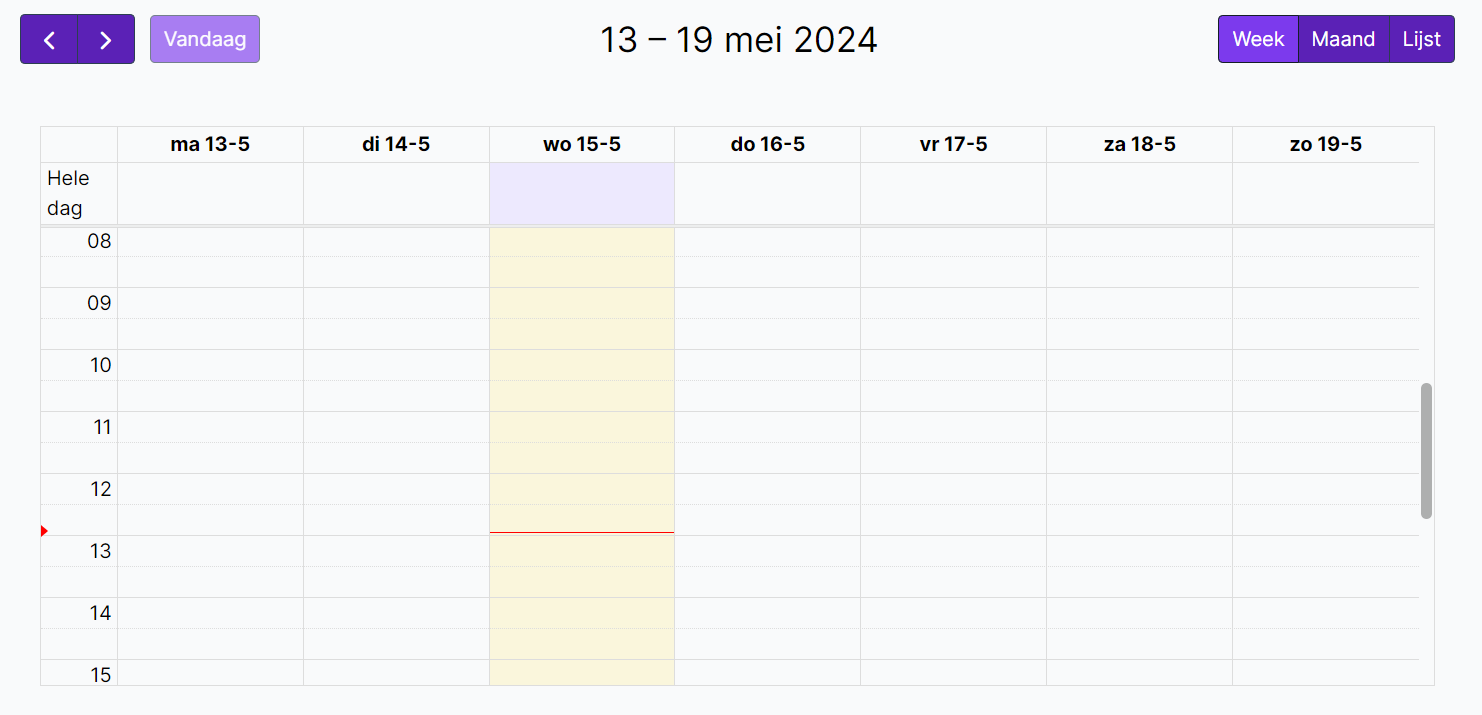
\includegraphics[width=\textwidth]{graphics/screenshot_kalender.png}
    \caption{Screenshot van de kalender.}
    \label{fig:screenshot_kalender}
\end{figure}


\subsubsection{Braindump}

Voor de Braindump zijn verschillende componenten gebruikt, waarbij gebruik is gemaakt van externe bibliotheken om deze correct te laten functioneren. Onder andere zijn een Drawer-, Dialog- en Sheet-component uit de MUI-bibliotheek geïmporteerd. Deze componenten worden ingezet om een venster aan de zijkant te laten verschijnen wanneer er op de desbetreffende ‘Braindump-knop’ wordt gedrukt. Op deze manier wordt de lay-out overzichtelijk gehouden en voorkomen we dat het te druk wordt.\newline

Voor de teksteditor die zich in dit uitklapbare venster bevindt, wordt gebruik gemaakt van de React Novel Lightweight-bibliotheek. Hiermee kan een ruimte gecreëerd worden die functionaliteiten biedt vergelijkbaar met Notion, waarbij het gevoel wordt gecreëerd alsof men op papier schrijft met de mogelijkheid tot het eenvoudig maken van lijsten, markeren, kleurcoderen, afbeeldingen invoegen, enzovoorts.\newline

Het implementeren van deze componenten ziet er als volgt uit: 

\begin{lstlisting}[language=JavaScript, caption={Code Snippet - Brain Dump Drawer}, label={lst:codesnippet2}, frame=single, breaklines=true, backgroundcolor=\color{lightgray}]
    
import Drawer from '@mui/joy/Drawer';
import ModalClose from '@mui/joy/ModalClose';
import DialogTitle from '@mui/joy/DialogTitle';
import DialogContent from '@mui/joy/DialogContent';
import Sheet from '@mui/joy/Sheet';
import Divider from '@mui/joy/Divider';
import BrainDumpEditor from '@/components//braindump/brainDumpEditor'


export default function BrainDumpDrawer({ openDrawer, setOpenDrawer }) {
    
    return (
    <Drawer
    open={openDrawer}
    onClose={() => setOpenDrawer(false)}
    anchor='right'
    size='lg'
    >
    
    <Sheet
    sx={{ /* Styling */ }}
    >
    <ModalClose />
    <DialogTitle>Brain Dump</DialogTitle>
    <Divider/>
    <DialogContent>
    <BrainDumpEditor />
    </DialogContent>
    </Sheet>
    </Drawer>
    )
    
}

\end{lstlisting}

\begin{lstlisting}[language=JavaScript, caption={Code Snippet - Text Editor}, label={lst:codesnippet3}, frame=single, breaklines=true, backgroundcolor=\color{lightgray}]
    
    import { Editor } from "novel-lightweight";
    import { useState } from "react";
    
    export default function BrainDumpEditor() {
        const [data, setData] = useState('');
        
        return (
        <Editor
        defaultValue={data}
        disableLocalStorage={false}
        onUpdate={(editor) => {
                setData(editor?.storage.markdown.getMarkdown());
        }}
        />
        );
    }
    
\end{lstlisting}

Het resultaat van de Braindump met volledige implementatie en gepaste styling ziet er als volgt uit (figuur 4.4):

\begin{figure}[h]
    \centering
    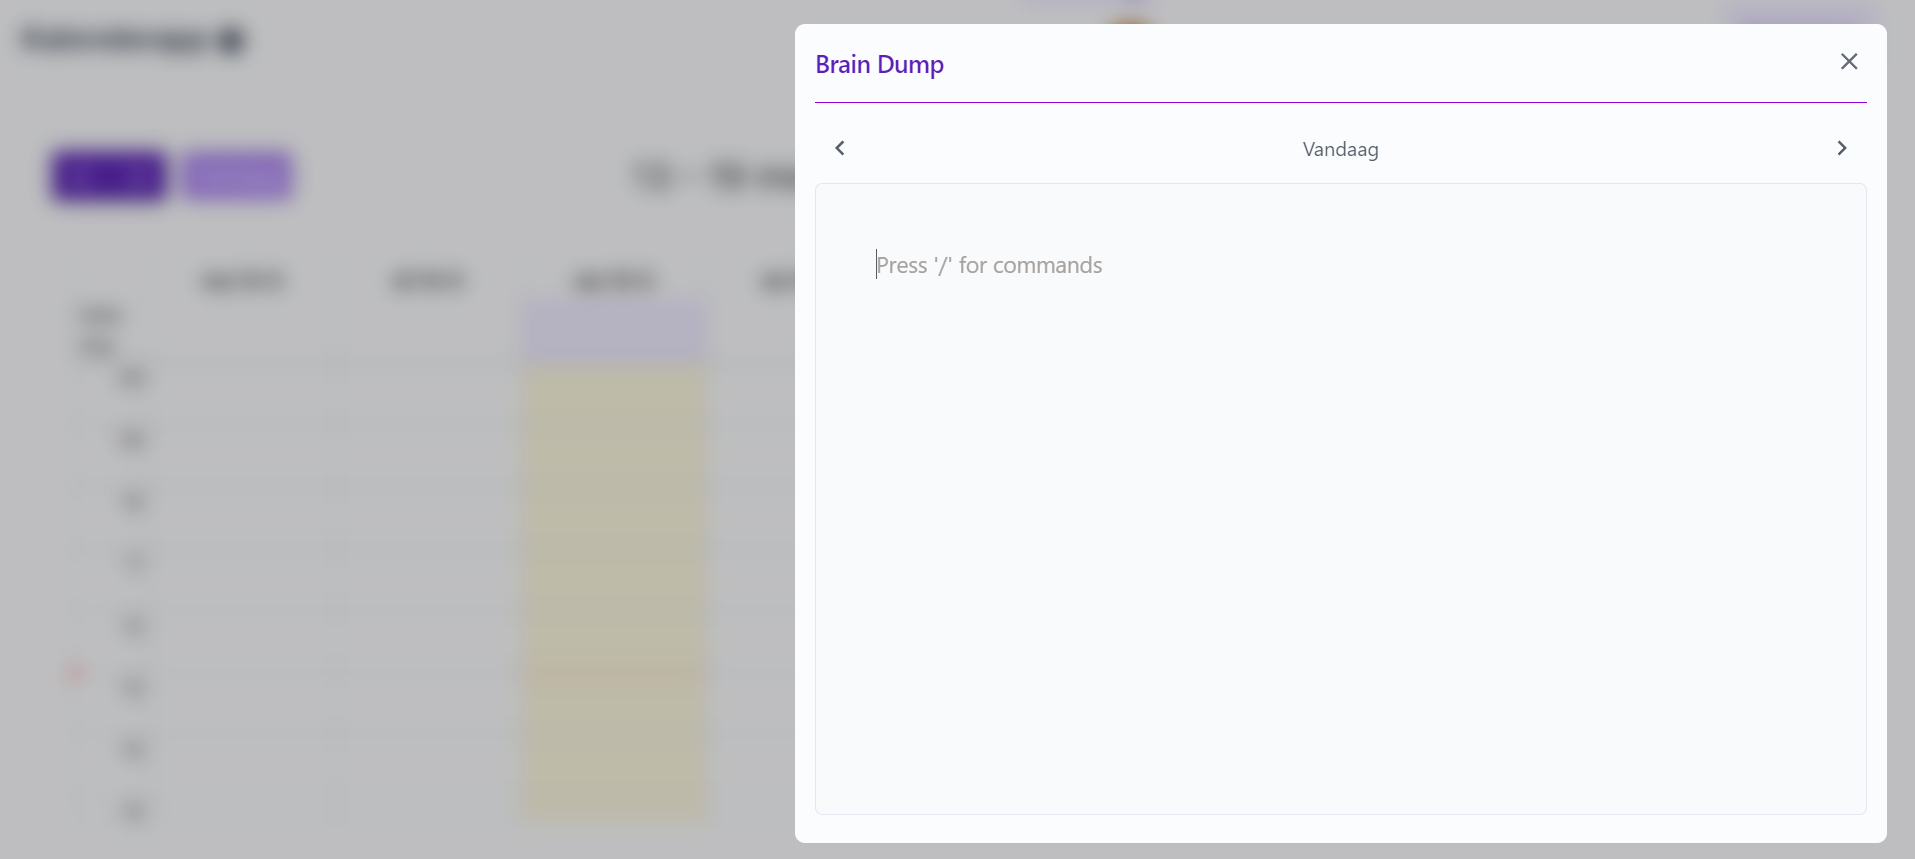
\includegraphics[width=\textwidth]{graphics/screenshot_braindump.png}
    \caption{Screenshot van de Brain Dump.}
    \label{fig:screenshot_braindump}
\end{figure}

\subsubsection{Overzicht in te plannen zaken}

Voor deze functionaliteit is geen nieuwe externe bibliotheek vereist; deze is volledig ontwikkeld met React-code en de 'Draggable'-eigenschap uit de FullCalendar-bibliotheek. Hoewel de code zelf niet wordt weergegeven in deze sectie, wordt een beschrijving gegeven van het uiteindelijke resultaat en hoe dit kan worden bereikt. \newline

Allereerst moet er naast de kalendercomponent een kader worden gecreëerd waarin de versleepbare evenementen geplaatst kunnen worden. Dit kan worden gerealiseerd met een `<div>`-element en passende opmaak. \newline

Dit kader wordt vervolgens gevuld door over een lijst van evenementen te mappen, waarbij voor elk element een blok wordt gegenereerd in de juiste kleur die overeenkomt met de categorie van het evenement. Deze blokken kunnen versleepbaar worden gemaakt door de klasse 'draggable-el' toe te wijzen aan het gegenereerde blok tijdens de iteratie over de lijst. \newline

Bij het laden van de pagina worden alle elementen met deze klasse omgezet in versleepbare objecten. Dit kan worden bereikt door gebruik te maken van de 'useEffect-hook' van React. Binnen deze hook worden de elementen gefilterd die behoren tot de gewenste klasse en worden ze omgezet naar versleepbare elementen met behulp van de 'new Draggable' methode uit de FullCalendar-bibliotheek. \newline

Het kader met overzicht van alle in te plannen zaken ziet er als volgt uit (figuur 4.5):

\begin{figure}[h]
    \centering
    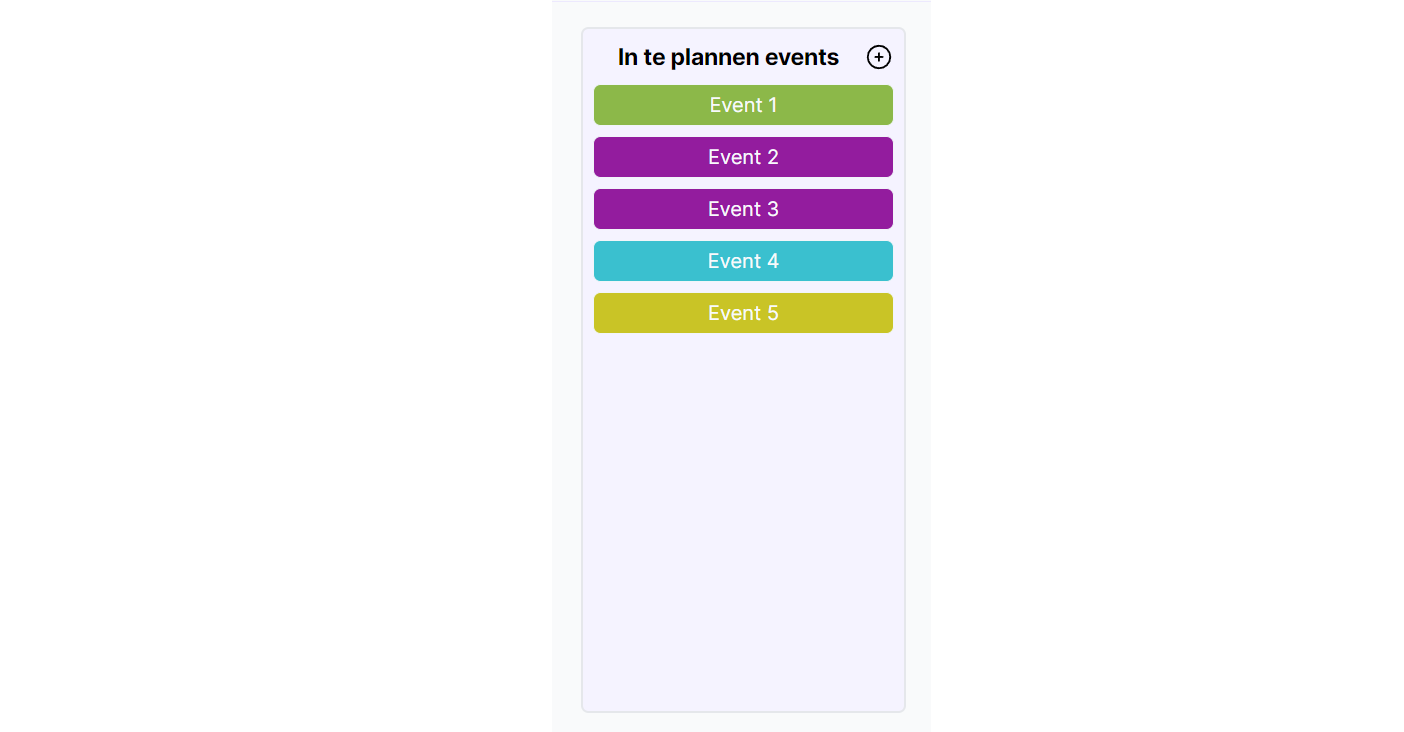
\includegraphics[width=\textwidth]{graphics/screenshot_overzicht.png}
    \caption{Screenshot van het Overzicht.}
    \label{fig:screenshot_overzicht}
\end{figure}


\subsubsection{Badges}

Als beloningssysteem in deze proof of concept zal een badgesysteem worden ontwikkeld. Dit systeem bestaat visueel uit een progressielijn tussen twee badges: de al verkregen badge van het vorige level en de te verkrijgen badge voor het volgende level. Daarboven zal er een knop aanwezig zijn die de verzameling behaalde badges toont, evenals een duidelijke weergave van het huidige level. \newline

Om dit op te zetten, is alleen het 'LinearProgress'-component van MUI nodig, terwijl de rest volledig kan worden ontworpen met React. \newline

De werking achter het badgesysteem in deze proof of concept is niet complex. Telkens wanneer een taak of evenement wordt voltooid, wordt deze toegevoegd aan een lijst. Op basis van deze lijst vordert de progressielijn. Zodra deze volledig is gevuld, gaat de gebruiker naar het volgende level en ontvangt deze een badge als beloning. Deze badge wordt ook toegevoegd aan de verzameling van de gebruiker, die te allen tijde kan worden geraadpleegd met behulp van de verzamelknop. \newline

Bij het halen van een nieuw level wordt de gebruiker ook gefeliciteerd en gemotiveerd om verder te doen. \newline

Hieronder vindt u de code voor het visualiseren van het badgesysteem, zonder styling.

\begin{lstlisting}[language=JavaScript, caption={Code Snippet - Badges}, label={lst:codesnippet4}, frame=single, breaklines=true, backgroundcolor=\color{lightgray}]
    <div>        
        <button onClick={() => setOpenCollection(true)}>
            Verzameling
        </button>
        <div>
            <Image alt="current" src={`/images/badgelvl${level}.png`}/>
            <LinearProgress variant="determinate" value={showProgressNumber} />    
            <Image alt="next" src={`/images/badgelvl${level + 1}.png`}/>
        </div>              
        <CongratulationDialog {...{ showCongratulations, setShowCongratulations, level }}/>
        <BadgeCollecion {...{ openCollection, setOpenCollection, level }}/>
    </div>
\end{lstlisting}

En hieronder krijgt u te zien hoe de progressielijn en motivatie eruitzien (figuur 4.6):

\begin{figure}[h]
    \centering
    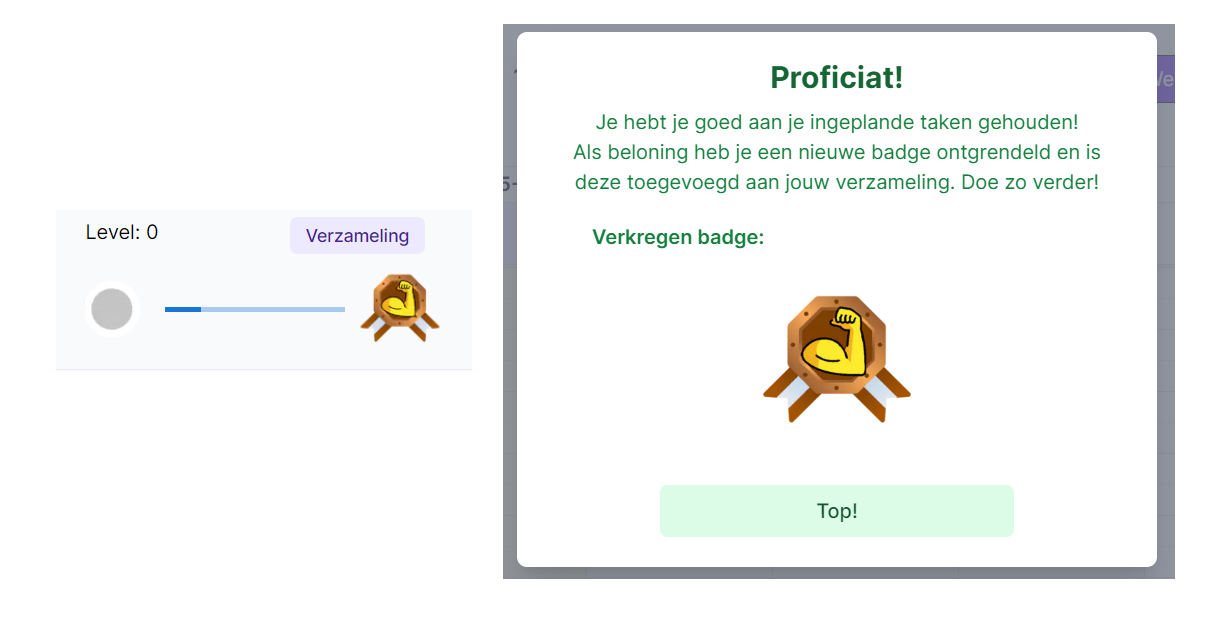
\includegraphics[width=\textwidth]{graphics/screenshot_badgesysteem.png}
    \caption{Screenshot van het Badgesysteem.}
    \label{fig:screenshot_badges}
\end{figure}


\subsubsection{Resultaat}
Als slot van deze sectie is er een screenshot van de gehele uitgewerkte applicatie (figuur 4.7). Nu dat deze volledig is uitgewerkt zal er in volgende sectie beschreven worden hoe deze applicatie getest zal worden in de praktijk. De resultaten van het onderzoek zullen later besproken en geïnterpreteerd worden.\newline
Figuur Proof of Concept: 

\begin{figure}[h]
    \centering
    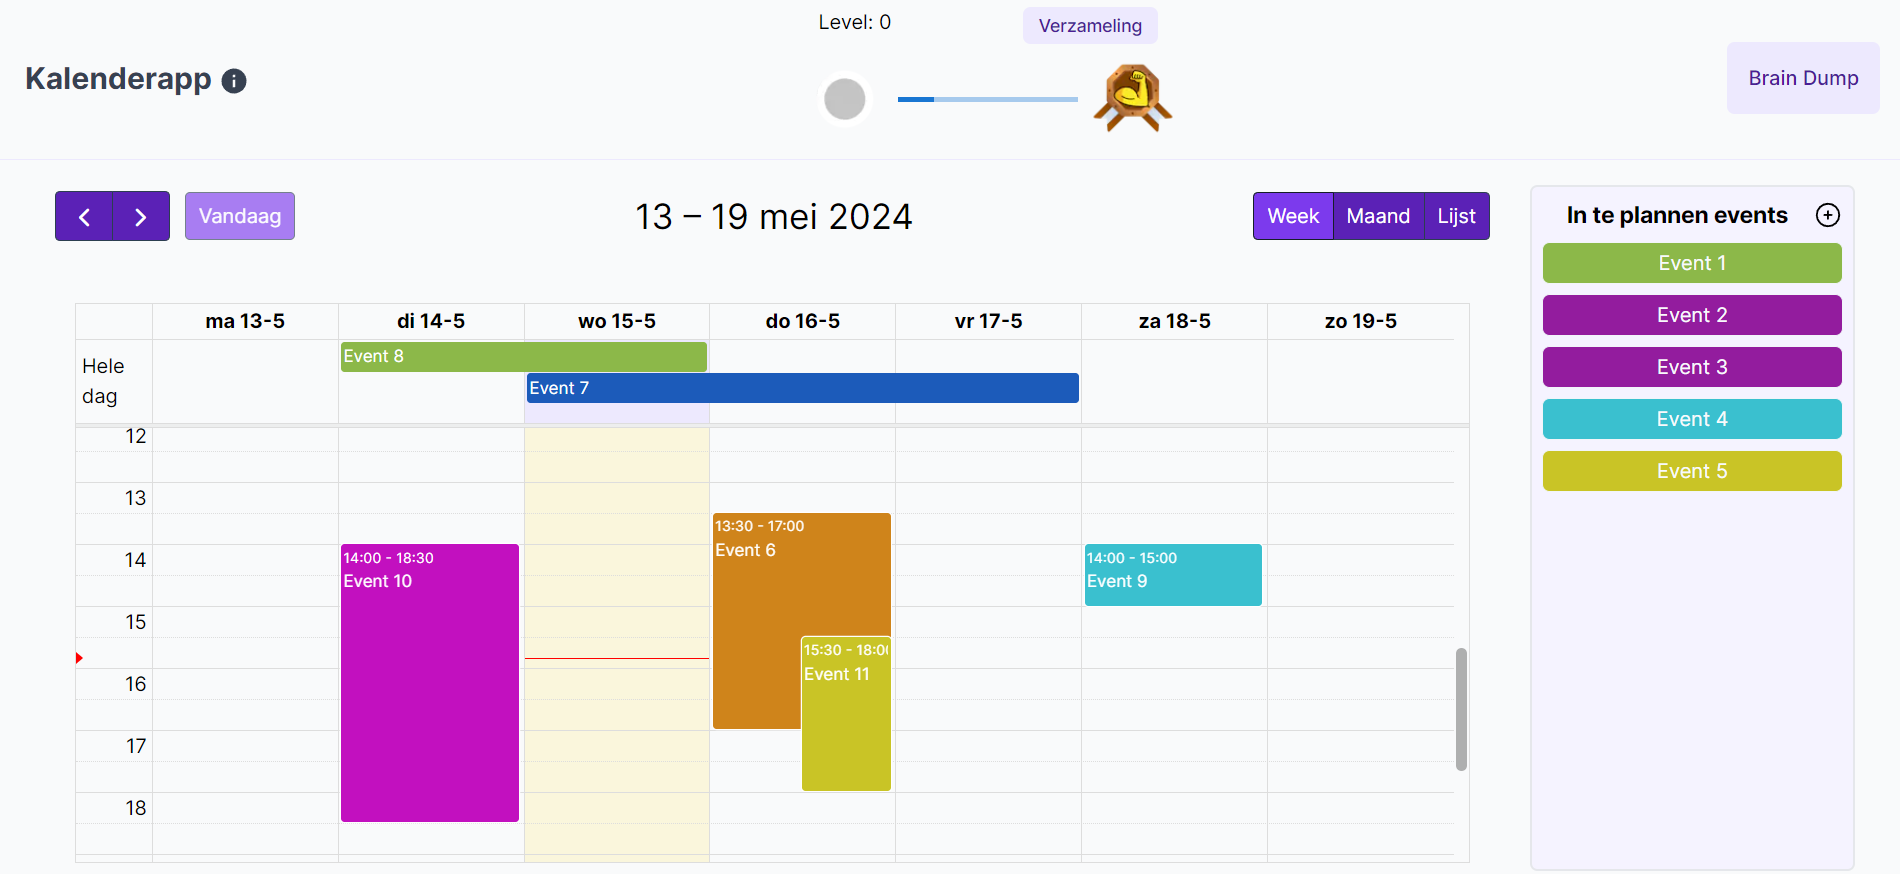
\includegraphics[width=\textwidth]{graphics/screenshot_applicatie.png}
    \caption{Screenshot van de Uitgewerkte Proof of Concept.}
    \label{fig:screenshot_applicatie}
\end{figure}

\subsection{Evaluatie van de applicatie}
Voor het testen van de proof of concept is er een evaluatieformulier opgesteld. Dit bevat bevragingen over de ontworpen features en de globale applicatie. Het formulier zal worden verspreid over de doelgroep die deze kritisch moet evalueren. In het formulier zit een link naar de applicatie die online draait en een handleiding om de applicatie volledig te kunnen testen. Er zal van de gebruikers verwacht worden om de aspecten en features een score te geven op 10. Er zal ook de mogelijkheid zijn om de kalenderapplicatie te vergelijken met een andere applicatie, die die de gebruiker op dit moment gebruikt bijvoorbeeld. Op basis van de scores en feedback zullen er conclusies worden getrokken. Dit is wat er in de volgende sectie zal gebeuren, het interpreteren van de resultaten.


